% !TEX root = ../memoria.tex

\chapter{Fundamentos teóricos}
\label{cap:capitulo3}



En este capítulo se presentan los fundamentos teóricos necesarios para entender el desarrollo del trabajo. Para poder abordar el reconocimiento de emociones mediante \ac{EEG}, primero es necesario conocer cómo se registran estas señales, qué información pueden aportar sus distintas bandas espectrales y qué relación pueden tener con la actividad emocional. Además, se introducen conceptos relacionados con el preprocesado de señales, el tratamiento de artefactos, el aprendizaje automático aplicado a \ac{EEG} y las técnicas utilizadas para interpretar los modelos obtenidos.

\section{Señales EEG y posicionamiento de electrodos}

La \ac{EEG} es una técnica que permite registrar la actividad eléctrica del cerebro mediante electrodos colocados en la cabeza. Lo que se mide realmente no es la actividad de una neurona aislada, sino pequeñas variaciones de voltaje generadas por la actividad conjunta de muchas neuronas, que llegan hasta la superficie de la cabeza y pueden ser captadas por los electrodos.

Estas señales suelen tener una amplitud muy baja, por lo que su registro requiere un equipo específico de adquisición y electrodos distribuidos por distintas zonas del cuero cabelludo. Dependiendo del dispositivo utilizado, los electrodos pueden necesitar gel o pasta conductora para mejorar el contacto con la piel, aunque también existen gorros que emplean electrodos secos o sensores humedecidos con agua mediante pequeñas esponjas.

Durante una grabación, el sujeto normalmente permanece sentado o en reposo mientras se registran las señales, y en estudios de emociones puede ser expuesto a estímulos como imágenes, sonidos o vídeos para observar cómo cambia la actividad cerebral. Aunque no siempre es obligatorio utilizar una sala médica específica, sí es recomendable realizar la grabación en un entorno controlado, cómodo y con las menores distracciones posibles, ya que factores como el movimiento, los parpadeos, la actividad muscular, la iluminación o la incomodidad pueden introducir ruido en la señal. Por este motivo, el registro no consiste únicamente en colocar electrodos y guardar datos, sino en intentar obtener una señal lo suficientemente limpia y controlada como para que posteriormente pueda analizarse y relacionarse con el estado mental o emocional del sujeto \cite{alarcao2019eeg}.


La corteza cerebral es una de las partes principales del cerebro y suele dividirse en cuatro lóbulos: frontal, temporal, parietal y occipital. Cada uno de ellos está relacionado con funciones diferentes. El lóbulo frontal participa en procesos asociados al pensamiento consciente; el temporal está relacionado con sentidos como el oído y el olfato, además del procesamiento de estímulos complejos como caras o escenas; el parietal integra información procedente de distintos sentidos y participa en la manipulación de objetos; y el occipital está principalmente vinculado con la visión \cite{alarcao2019eeg}. Aunque la grabación no permita localizar con precisión exacta la actividad de cada región cerebral, la posición de los electrodos ofrece una referencia aproximada de la zona desde la que se está registrando la señal.

\begin{figure}[H]
    \centering
    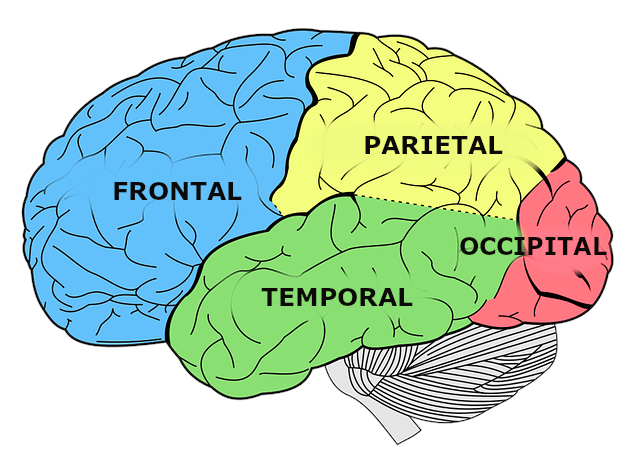
\includegraphics[width=0.55\textwidth]{figs/lobulos_cerebrales.png}
    \caption{Principales lóbulos de la corteza cerebral. Fuente: \cite{psycolab2021lobulos}.}
    \label{fig:lobulos_cerebrales}
\end{figure}


La colocación de los electrodos no se realiza de forma aleatoria, sino siguiendo sistemas estandarizados que permiten registrar la actividad cerebral de manera ordenada y comparable entre sujetos. Uno de los sistemas más utilizados es el sistema internacional 10-20, en el que las posiciones de los electrodos se calculan a partir de referencias anatómicas de la cabeza, como el nasion, el inion y los puntos preauriculares. El nombre 10-20 hace referencia a que las distancias entre posiciones se establecen como porcentajes del tamaño de la cabeza, lo que permite adaptar el montaje a cada persona. Además, existen sistemas más densos, como el sistema 10-10 o el montaje estándar 10-05, que añaden posiciones intermedias y permiten trabajar con configuraciones de mayor número de electrodos. En la práctica, los registros de \ac{EEG} pueden realizarse con montajes de distinta densidad, como 32 o 64 electrodos. Un montaje de 32 canales puede ofrecer una cobertura general, mientras que uno de 64 canales permite recoger información con mayor detalle espacial. \cite{klem1999tentwenty,oostenveld2001five}.


\begin{figure}[H]
    \centering
    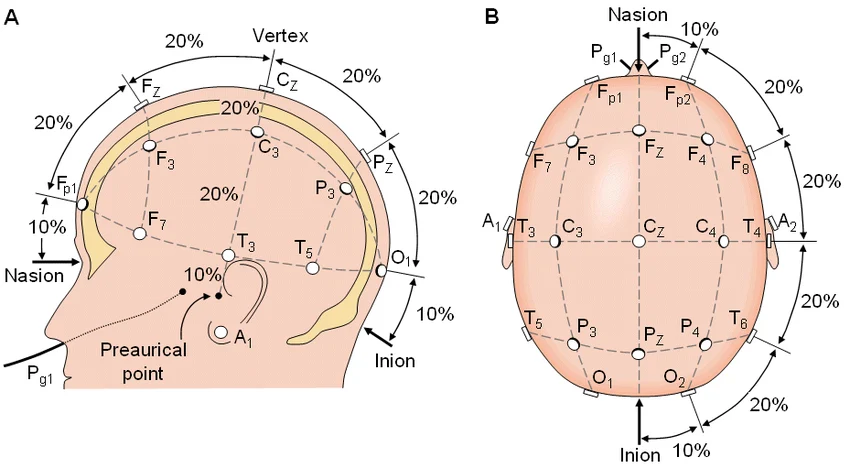
\includegraphics[width=0.65\textwidth]{figs/sistema_10_20.png}
    \caption{Sistema internacional 10-20 para la colocación de electrodos EEG. Fuente: \cite{novo2010mapeo}.}
    \label{fig:sistema_10_20}
\end{figure}

La nomenclatura de los electrodos indica la zona aproximada en la que se encuentran: F a la frontal, C a la central, T a la temporal, P a la parietal y O a la occipital. Además, la letra z indica posiciones situadas en la línea media, los números impares suelen corresponder al hemisferio izquierdo y los pares al hemisferio derecho. Esta localización es importante porque cada canal recoge información de una zona concreta, por lo que la posición de los electrodos influye directamente en el análisis posterior, especialmente cuando se estudia qué canales o regiones tienen más importancia en la clasificación de emociones.

\section{Bandas espectrales}

La señal de \ac{EEG} puede analizarse tanto en el dominio temporal como en el dominio frecuencial. En este segundo caso, la señal se descompone en distintos rangos de frecuencia, conocidos como bandas espectrales. Estas bandas permiten estudiar qué parte de la actividad cerebral aparece con mayor presencia en cada momento y facilitan la extracción de características para su posterior uso en modelos de aprendizaje automático. Aunque los límites exactos pueden variar ligeramente según el autor, normalmente se distinguen cinco bandas principales: delta, theta, alpha, beta y gamma \cite{alarcao2019eeg}.

\begin{table}[H]
\centering
\begin{tabular}{|c|c|p{7cm}|}
\hline
\textbf{Banda} & \textbf{Rango aproximado} & \textbf{Asociación general} \\
\hline
Delta & 1--4 Hz & Se suele relacionar con estados de sueño profundo o baja actividad consciente. \\
\hline
Theta & 4--8 Hz & Se asocia a estados de somnolencia, relajación o actividad subconsciente. \\
\hline
Alpha & 8--12 Hz & Suele aparecer en estados de relajación, especialmente cuando la persona está despierta pero tranquila. \\
\hline
Beta & 12--30 Hz & Se relaciona con estados de mayor actividad mental, atención o concentración. \\
\hline
Gamma & $>$30 Hz & Se asocia con una actividad cerebral más intensa o procesos de integración de información. \\
\hline
\end{tabular}
\caption{Bandas espectrales principales de la señal EEG.}
\label{tab:bandas_eeg}
\end{table}

El análisis por bandas es importante porque muchas veces la información relevante de una señal de \ac{EEG} no se encuentra directamente en la señal completa, sino en cómo cambia la actividad dentro de determinados rangos de frecuencia. Por ejemplo, en lugar de utilizar únicamente la señal cruda, es habitual calcular características como la potencia de cada banda en distintos canales. De esta forma, el modelo puede trabajar con una representación más compacta y útil de la actividad cerebral.

En el reconocimiento de emociones, estas bandas pueden aportar información relevante, ya que la actividad alpha y la asimetría entre hemisferios se han relacionado con la valencia emocional, mientras que las bandas beta y gamma también aparecen asociadas a la diferenciación de ciertos estados afectivos \cite{alarcao2019eeg}. Por este motivo, en trabajos de clasificación emocional con \ac{EEG} es frecuente extraer características a partir de varias bandas espectrales, ya que cada una puede aportar información distinta sobre la respuesta cerebral.


\section{Emociones y actividad cerebral: alegría, tristeza y estado neutro}

Las emociones pueden representarse de distintas formas. Una de ellas es mediante modelos discretos, donde cada emoción se trata como una categoría concreta, por ejemplo alegría, tristeza, miedo o ira. Otra forma habitual es utilizar modelos dimensionales, en los que las emociones se describen a partir de ejes continuos. Uno de los modelos más utilizados es el de valencia-excitación, donde la valencia indica si la emoción es más positiva o negativa, mientras que la excitación representa el nivel de activación asociado a esa emoción. Desde esta perspectiva, la alegría puede situarse en una zona de valencia positiva, la tristeza en una zona de valencia negativa y el estado neutro en una posición más intermedia, con una carga emocional menos marcada \cite{alarcao2019eeg}.

\begin{figure}[H]
    \centering
    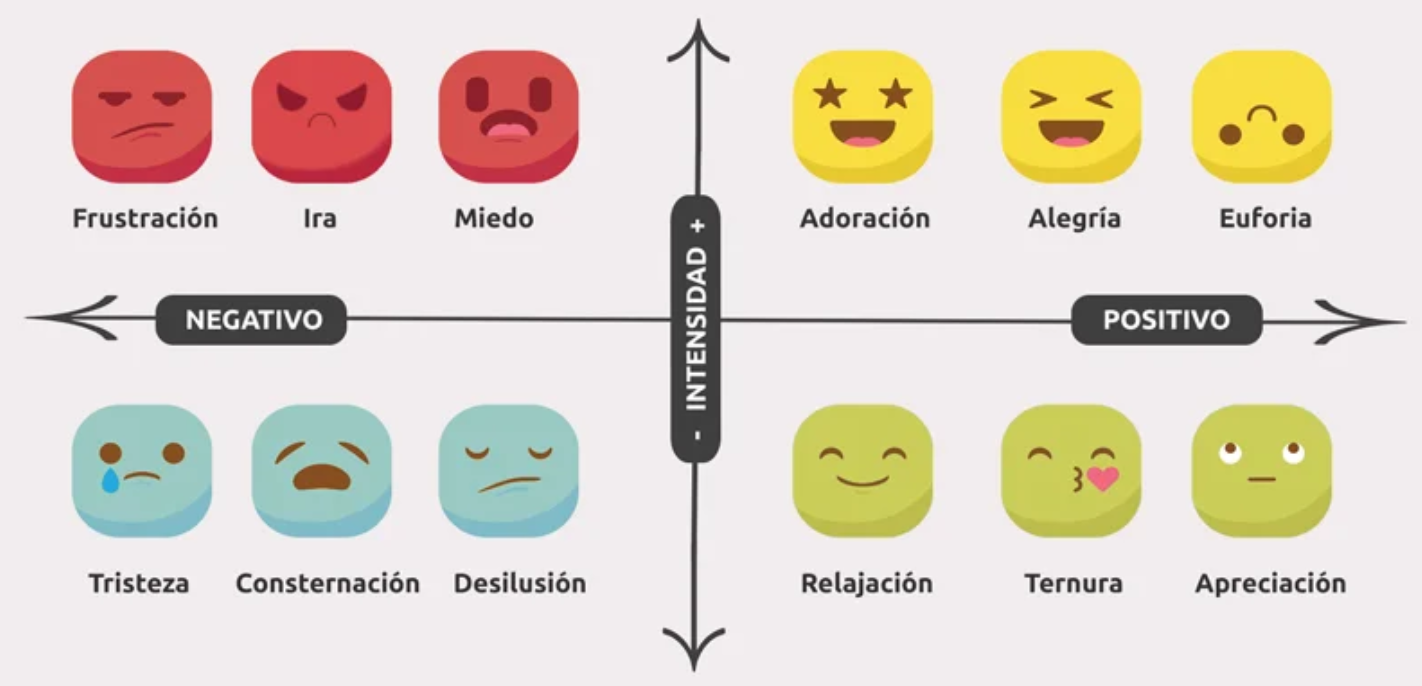
\includegraphics[width=0.60\textwidth]{figs/valencia_activacion.png}
    \caption{Representación simplificada de emociones según valencia y arousal. Adaptado de \cite{rinconpsicologia2024emociones}.}
    \label{fig:modelo_valencia_arousal}
\end{figure}

Para detectar estados emocionales a partir de señales de \ac{EEG}, los estudios 
analizan cómo varía la actividad cerebral en distintas regiones ante diferentes estímulos, siendo las zonas frontal y parietal las que aparecen con mayor frecuencia como relevantes \cite{alarcao2019eeg}. A partir de estas 
observaciones, se extraen características de la señal que se utilizan como entrada a modelos de clasificación. Sin embargo, estas relaciones no constituyen patrones universales, sino tendencias que varían considerablemente entre personas: la respuesta cerebral ante una misma emoción puede diferir de forma notable de un sujeto a otro. Esta variabilidad intersujeto es uno de los principales retos del campo y explica por qué los modelos entrenados con datos de varios sujetos no siempre generalizan bien, lo que justifica también el análisis de modelos individuales por sujeto \cite{rajpoot2022subject}.

De forma general, las emociones positivas suelen asociarse con una mayor actividad relativa en regiones frontales izquierdas, mientras que las emociones negativas se han relacionado con una mayor actividad relativa en regiones frontales derechas. Esta diferencia entre hemisferios se conoce como asimetría frontal y se ha utilizado en distintos estudios como una posible señal relacionada con la valencia emocional. El estado neutro no debería presentar una activación emocional tan marcada, por lo que puede utilizarse como referencia frente a las emociones con mayor carga afectiva \cite{alarcao2019eeg}.

\section{Técnicas de explicación}


Para analizar el comportamiento de los modelos entrenados, en este trabajo se emplean dos tipos de técnicas de explicación: los valores \ac{SHAP} y los mapas topográficos. Ambas permiten examinar, desde perspectivas distintas, qué información de la señal de \ac{EEG} tiene más peso en las decisiones del clasificador.

Los mapas topográficos, o \textit{topomaps}, permiten representar información de la señal de \ac{EEG} sobre una distribución espacial similar a la posición real de los electrodos en el cráneo. De esta forma, es posible visualizar qué zonas presentan mayor actividad o mayor importancia dentro del análisis realizado. En el reconocimiento de emociones, es habitual generar un mapa por cada banda espectral analizada, ya que la importancia de cada región puede variar en función de la frecuencia. Además, los valores representados pueden interpretarse en valor absoluto, indicando la magnitud de la contribución de cada zona, o con signo, mostrando si esa contribución empuja hacia una clase o la aleja. Los \textit{topomaps} permiten comparar visualmente los patrones asociados a alegría, tristeza y estado neutro a lo largo de las distintas bandas espectrales.


\begin{figure}[H]
    \centering
    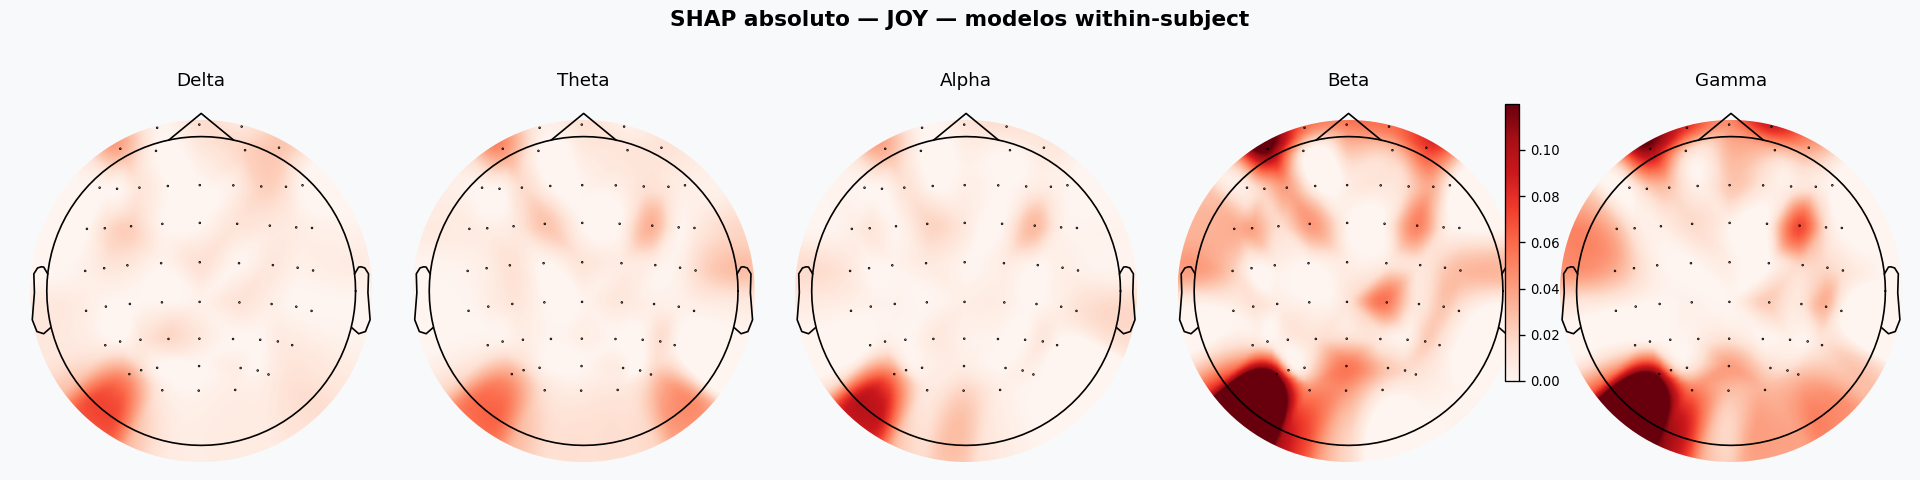
\includegraphics[width=\textwidth]{figs/topomap_ejemplo.png}
    \caption{Ejemplo de topomaps por banda espectral para la clase alegría.}

    \label{fig:topomap_ejemplo}
\end{figure}

Por otro lado, \ac{SHAP} es una técnica de explicación basada en la teoría de juegos cooperativos que asigna a cada característica un valor según cuánto contribuye a la predicción del modelo. Su principal ventaja es que ofrece explicaciones tanto a nivel global, mostrando qué variables son más relevantes en general, como a nivel individual, indicando en qué dirección empuja cada característica una predicción concreta. En modelos lineales, este valor puede calcularse de forma exacta a partir de los coeficientes del modelo, sin necesidad de aproximaciones \cite{lundberg2017shap}.

\begin{figure}[H]
    \centering
    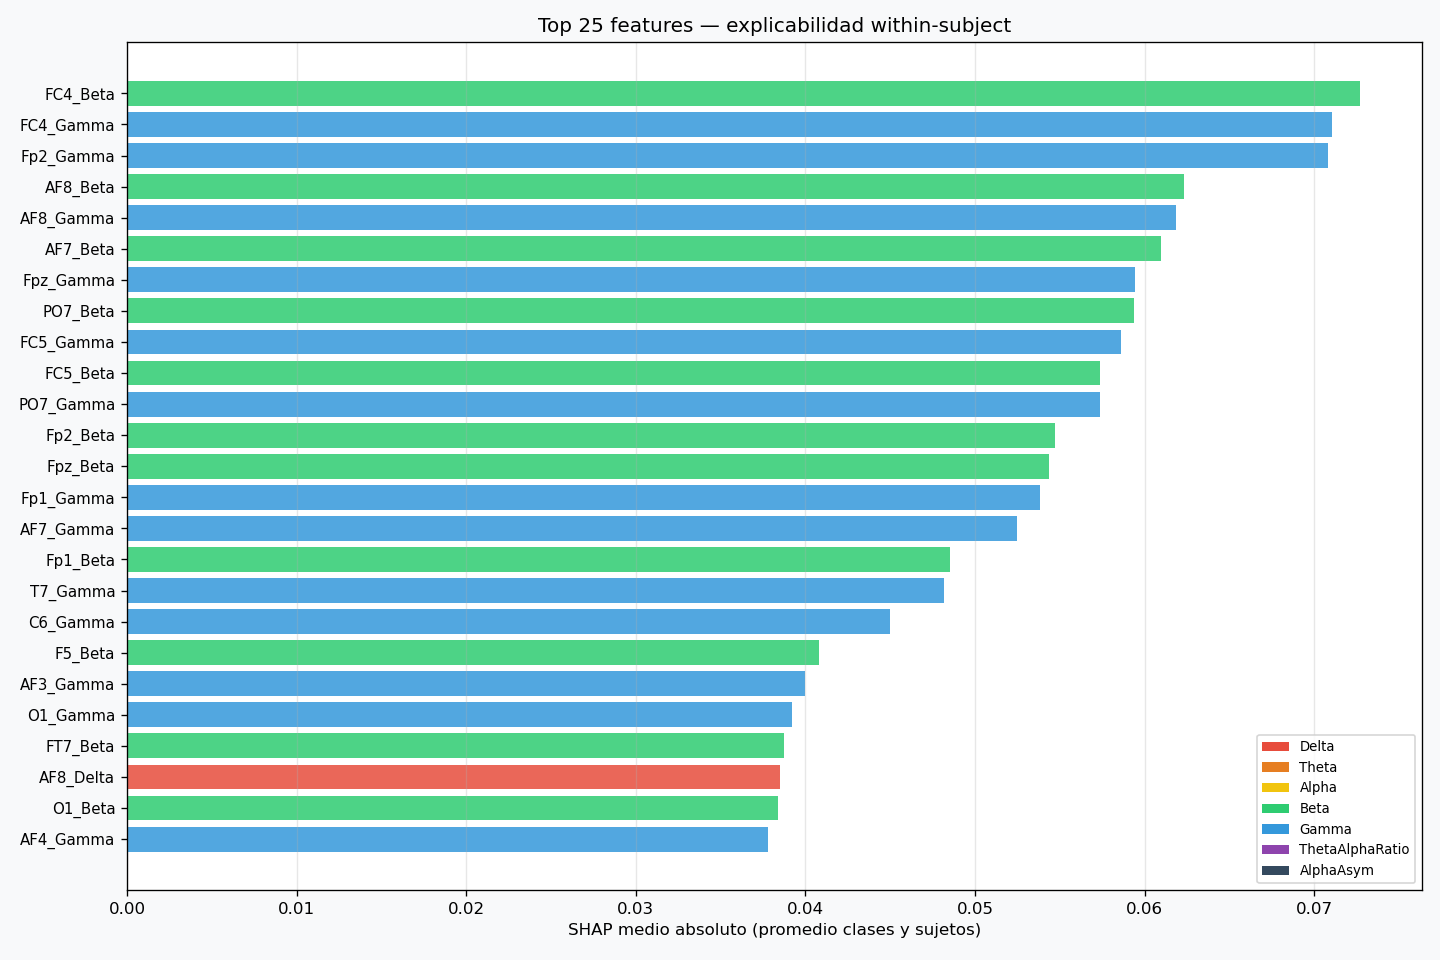
\includegraphics[width=0.85\textwidth]{figs/shap_ejemplo.png}
    \caption{Ejemplo de importancia de características mediante valores SHAP.}
    \label{fig:shap_ejemplo}
\end{figure}

\section{Aprendizaje automático aplicado a EEG}
\subsection{Modelos de caja negra frente a modelos interpretables}
\subsection{Clasificadores}
\subsection{Estrategia de evaluación y validación cruzada}
\subsection{Métricas}


